%%%%%%%%%%%%%%%%%%%%%%%%%%%%%%%%%%%%%%%%%%%%%%%%%%%%%%%%%%%%%%%%%%%%%%%%
% Plantilla TFG/TFM
% Escuela Politécnica Superior de la Universidad de Alicante
% Realizado por: Jose Manuel Requena Plens
% Contacto: info@jmrplens.com / Telegram:@jmrplens
%%%%%%%%%%%%%%%%%%%%%%%%%%%%%%%%%%%%%%%%%%%%%%%%%%%%%%%%%%%%%%%%%%%%%%%%
\chapter{Introduction}

This chapter will introduce the reader to the context of this project. It
starts by providing a succinct overview of the problem at hand, followed by a
detailed discussion of the motivation underpinning this work. Lastly, it will
provide an outline of the subsequent chapters in the document.

\section{Motivation and Context}

Obesity poses a significant global public health concern, affecting a
substantial segment of the global population. \todo{Elaborate on why obesity is
	a pressing issue}.

Tech4Diet is a research project that seeks to understand how obesity treatments
induce morphological changes in the human body. \todo{Provide more details
	about Tech4Diet}

In a previous initiative, \todo{Provide a reference link} Tech4Diet developed a
system that allowed patients undergoing weight loss treatment to visualize 3D
scans of their bodies throughout their journey~\cite{Azorin-Lopez2020}.

During the treatment, the patient's body is captured using an RGBD camera,
specifically the Intel RealSense D435. The 3D model of the human body is
displayed during different sessions using a virtual reality headset. This
innovative approach was designed to enhance motivation and boost adherence to
the treatment plan.

\begin{figure}
	\centering
	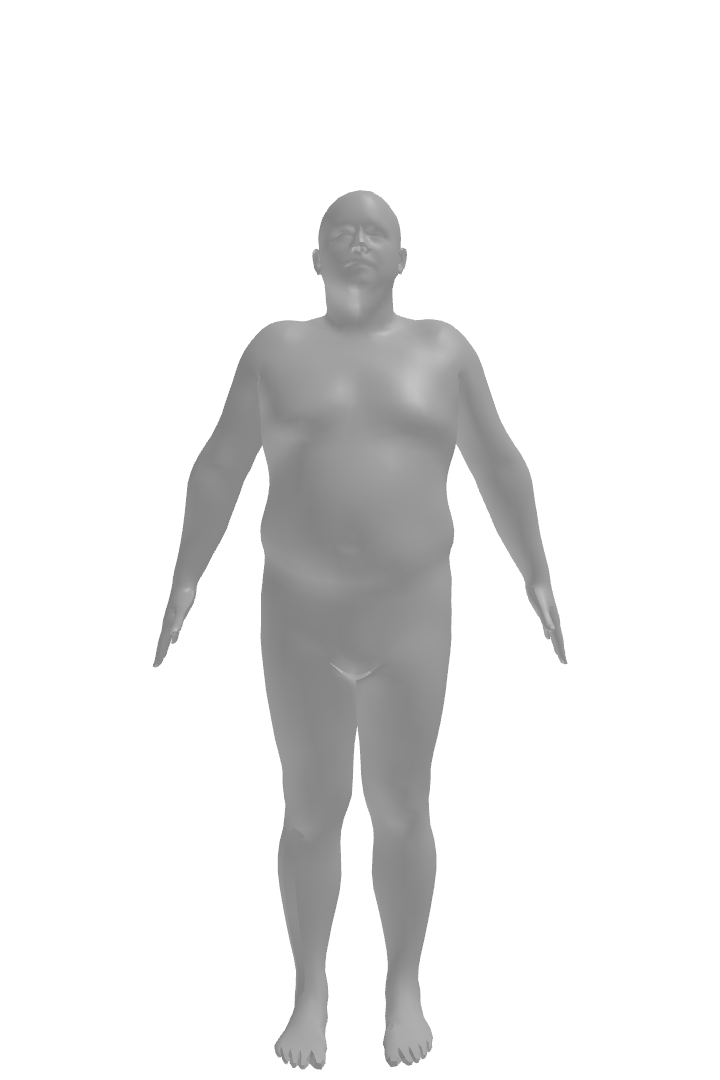
\includegraphics[width=75pt]{files/patient_8/8_2}
	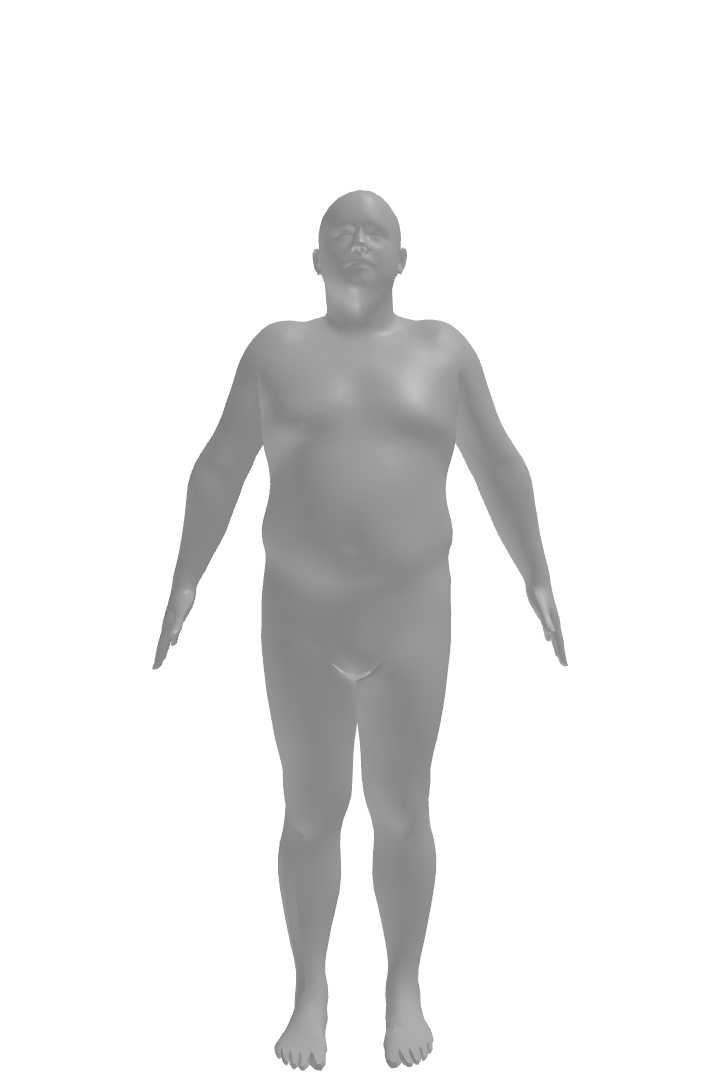
\includegraphics[width=75pt]{files/patient_8/8_3}
	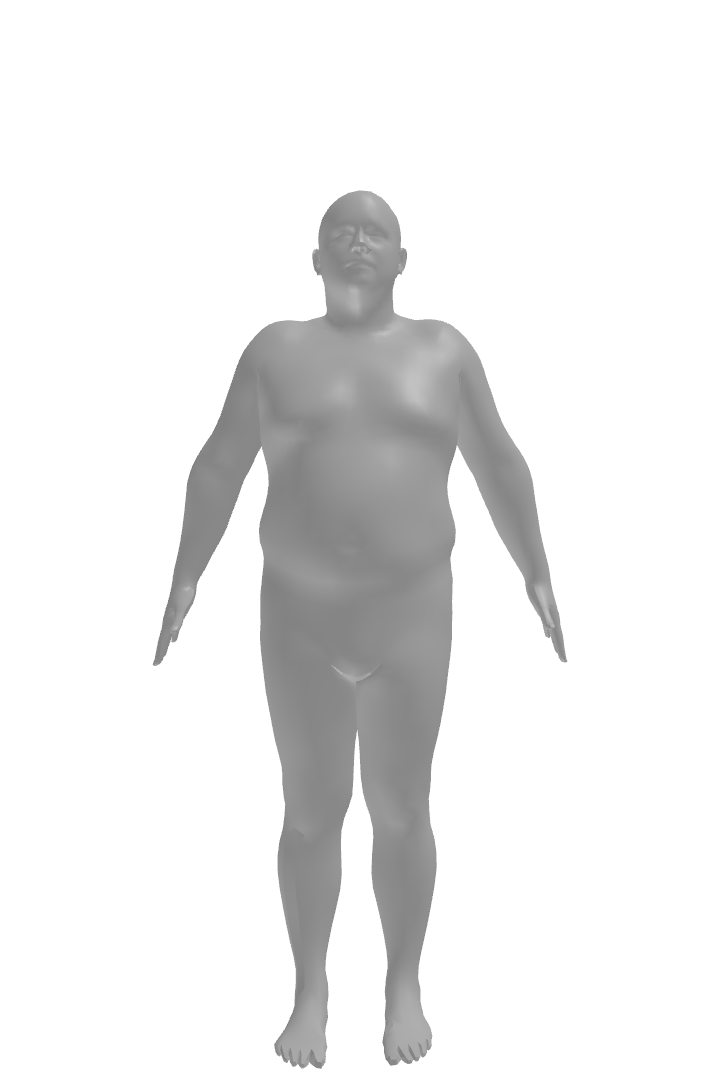
\includegraphics[width=75pt]{files/patient_8/8_4}
	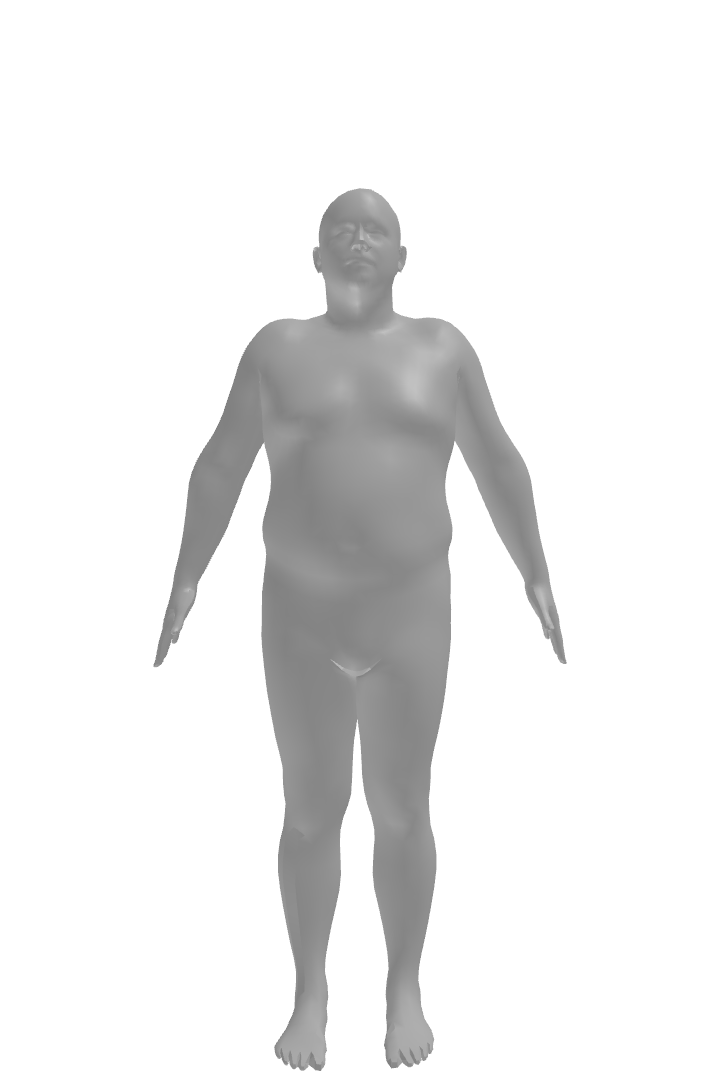
\includegraphics[width=75pt]{files/patient_8/8_5}
	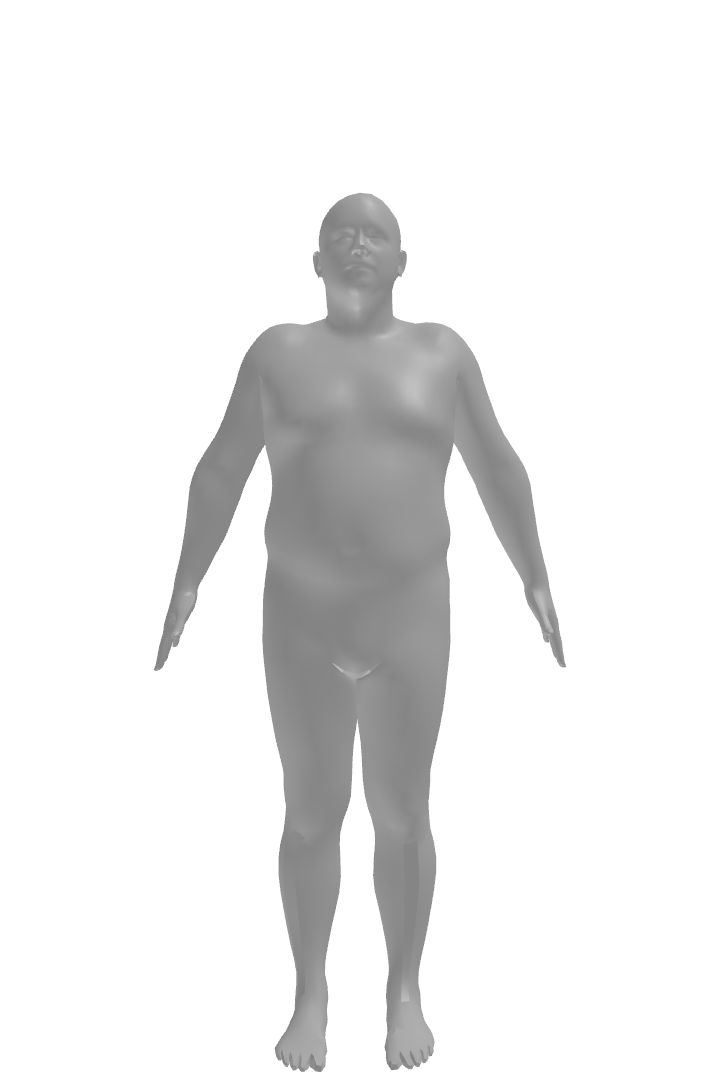
\includegraphics[width=75pt]{files/patient_8/8_6}
	\caption[Reconstructed 3D body of a patient's scans]{3D model reconstruction of a patient's body at different stages of a weight loss
		treatment. Each scan is taken approximately a month apart, with a total
		weight loss of 3.8 kg.}
\end{figure}

Apart from body scans, the study also collated other medical data, including
variables such as weight, localized fat and muscle mass, activity levels, and
psychological factors.

Building on this, we sought to explore the feasibility of using the datasets
acquired from this prior study to develop a predictive model. The intention was
for this model to forecast changes in a person's body undergoing weight loss
treatment before the treatment concludes, thereby bolstering adherence to the
treatment regimen.

The present work encapsulates the development of such a model. This encompasses
analyzing data from the earlier study, examining existing techniques in human
body model representation, encoding patient data using the selected
representation, designing a neural network architecture for predicting patient
body changes, training, and evaluating the model. Ultimately, the model
generates 3D meshes of the predicted body changes.

The following chapters will delve into the details of this process. Chapter
\ref{chap:data} discusses the data collected during the previous study, and how
we prepared it for use in our model. It also presents how we encoded the human
body scans. Chapter \ref{chap:nn} reviews the neural network architecture we
formulated for this project, including the training process and the results
obtained. Chapter \ref{chap:results} interprets the results of our model, and
chapter \ref{chap:conclusion} concludes the document by summarizing the work
done and suggesting possible future lines of research.

\section{Background}

In this section, we provide a comprehensive overview of the state-of-the-art
methodologies for human body representation, the generation of these models,
and the deployment of generative neural networks. The knowledge derived from
these studies has paved the way for our submission to the \gls{iwann} 2023
conference. \todo{link}

\subsection{3D Human Body Representation}

Advancements in 3D human body recovery have largely been driven by the
development of parametric models. These models use sets of parameters to
represent body shape and pose, becoming instrumental in the reconstruction of
3D human bodies. They vary in focus—some emphasize body deformations, others
shape and pose optimization, while others separate body shape into
identity-specific and pose-dependent components. Each approach has its own
advantages and applications, contributing to improved accuracy and stability in
representing human body shapes and poses.

Broadly speaking, human body representations can be categorized based on the
required input type and the resulting output:

\subsubsection{Input Types}

\begin{itemize}
	\item \textbf{2D input:} Models that utilize 2D images or videos as input.
	\item \textbf{3D input:} Models that require 3D point clouds as input data.
	\item \textbf{Parametric models:} Models that require a set of parameters describing the body.
\end{itemize}

\subsubsection{Output Types}

\begin{itemize}
	\item \textbf{3D meshes:} Models that generate a 3D mesh of the body.
	\item \textbf{3D voxel:} Models that produce a 3D voxel grid of the body.
	\item \textbf{\gls{nerf}:} Models that render the object directly from a specific viewpoint.
\end{itemize}

\subsection{Generation of 3D Human Body Models}

In the realm of 3D human model generation, two primary approaches exist. One
uses a general-purpose generator system guided to generate human models. The
second deploys a generator specifically designed for creating human models from
the beginning.

\subsubsection{Human-Specific Generators}

Human-specific generators have gained considerable attention in recent years,
with several notable examples:

\begin{itemize}
	\item \textbf{SMPLify} \cite{SMPLify} is a method for estimating 3D human pose and shape from a single image.
	\item \textbf{SiCloPe} \cite{SiCloPe} models clothed human bodies using deep generative models.
	\item \textbf{PIFu} and \textbf{PIFuHD} \cite{PIFu, PIFuHD} are effective implicit representations aligning 2D image pixels with their corresponding 3D object.
	\item \textbf{Tex2Shape} \cite{Tex2Shape} infers detailed full human body shape from a single photograph.
	\item \textbf{HumanMeshNet} \cite{HumanMeshNet} and \textbf{DeepHuman} \cite{DeepHuman} focus on 3D human body reconstruction from a monocular image.
	\item \textbf{HumanGen} \cite{humangen} provides a detailed 360° realistic free-view rendering of the human body.
	\item \textbf{HumanNeRF} \cite{humannerf} offers a high-fidelity free-view synthesis of dynamic humans.
\end{itemize}

\subsubsection{General Purpose Generators}

For general-purpose generators, \textbf{CoCosNet} and its second version
\cite{CoCosNet, CoCosNet2} have shown significant effectiveness in cross-domain
image translation.

\subsection{Parametric Models}

Parametric models for representing and generating 3D human body shapes and
poses have gained significant interest in recent years. These models are based
on adjustable parameters that allow for pose and shape modifications, enabling
the reconstruction and creation of unique human bodies. They find applications
in animation, virtual reality, and garment simulation.

One notable early work in this field is Allen's method, which utilizes a
statistical model to create a parametric model of the human body. It matches
the pose of a human in a 3D scan by interpolating from example scans with
similar joint angles. However, it does not account for how body shape changes
with pose, primarily serving as a hole-filling technique.

Another significant model is SCAPE, which represents body deformations caused
by shape and pose as triangle deformations. It uses linear regression to
determine pose deformations. Although it aims to represent muscle deformations,
it lacks specificity for different muscle activities and fails to capture
motion-related tissue perturbations.

BlendSCAPE extends the SCAPE model by optimizing shape and pose registration
simultaneously using a blending technique. However, its formulation is
incompatible with standard graphics packages and may not be suitable for common
graphics applications.

SymmetricSCAPE, a variant of SCAPE and BlendSCAPE, incorporates symmetry
constraints to enhance the accuracy and stability of the model, resulting in a
more robust representation of the 3D human body.

The SMPL model is widely used for 3D human body shape and pose representation.
It separates body shape and pose into parameters and employs a vertex-based
skinning approach with corrective blend shapes, offering greater flexibility.
It is compatible with various graphics applications.

Improvements to the SMPL model include SMPL-H, which incorporates articulated
hand pose and shape parameters, and SMPL-X, which includes hand and face pose
and shape parameters.

The STAR model addresses limitations of SMPL, such as reducing mesh volume
around joints, by learning corrective blend shapes. It offers realistic
deformations of the 3D human body while requiring fewer parameters than SMPL.

Another approach is presented in BLSM, which utilizes a bone-level skinning
method. It establishes the skeleton first by determining bone lengths and
angles, incorporating identity-specific variations, and then applies linear
blend skinning for animation.

\todo{add citations}

\subsection{Generative Neural Networks}

Finally, generative neural networks such as Variational Autoencoders (VAEs) and
Generative Adversarial Networks (GANs) have emerged as powerful tools for
generating 3D models of the human body. They learn the distribution of the data
and generate 3D human body models accordingly. They are widely applicable
across various fields, including medicine, film and video game industries,
extended reality, and clothing.

This general overview of the current state-of-the-art methodologies forms the
foundation upon which we build our research. The following sections delve into
our unique approach and the results obtained from our experiments.

\section{Neural Network Architectures}\todo{}

\section{Objectives}\label{objectives}

This project is guided by the following objectives. They are designed to
provide a clear structure for the work and ensure that the project's goals are
achieved, as well as serving for the author to develop a deeper understanding
of the subject matter.

\begin{itemize}
	\item \textbf{Objective 1: Comprehensive Literature Review}
	      \begin{itemize}
		      \item Understand the current state of the art in human body representation and
		            generation.
		      \item Critically analyze the advantages and disadvantages of existing methodologies.
		      \item Identify the most promising approach to guide our project.
	      \end{itemize}

	\item \textbf{Objective 2: Data Preparation}
	      \begin{itemize}
		      \item Conduct a thorough exploration of the project's data and understand its
		            characteristics.
		      \item Implement rigorous preprocessing steps to ensure the data's quality and
		            consistency.
		      \item Investigate potential data augmentation techniques to enhance the robustness of
		            our models.
	      \end{itemize}

	\item \textbf{Objective 3: Neural Network Development}
	      \begin{itemize}
		      \item Survey potential neural network architectures suitable for time series
		            prediction problems.
		      \item Design a bespoke neural network architecture that is optimized for future human
		            body shape generation.
		      \item Implement and train the proposed neural network, fine-tuning its parameters for
		            optimal performance.
		      \item Evaluate the predictive performance of our trained network.
	      \end{itemize}

	\item \textbf{Objective 4: Result Evaluation}
	      \begin{itemize}
		      \item Generate human body shape predictions using our past data.
		      \item Conduct an evaluation of our model's predictive performance, discussing its
		            potential applications and limitations.
	      \end{itemize}

\end{itemize}
